\section{Lecteur de cartes}
\begin{frame}{Besoin et solutions}
	\begin{block}{Besoin}
        Besoin de savoir de façon rapide et efficace l'assiduité des élèves aux 
        conférences. Nécessite donc une identification unique.
	\end{block}

	\begin{block}{Solution}
	    \begin{itemize}
            \item Money Kart
            \item Cartes étudiantes
	    \end{itemize}
	\end{block}
\end{frame}


\subsection{RFID et Mifare}
\begin{frame}{RFID et Mifare}
	\begin{block}{RFID}
        La radio-identification qui permet de mémoriser et d'envoyer des données sur
        de courtes distances.

	    \begin{itemize}
            \item Tamway de Montpellier
            \item Cartes étudiantes de l'UM2
	    \end{itemize}
	\end{block}

	\begin{block}{Mifare}
        Différents types de données souvent stockées sur les cartes étudiantes par
        exemples. Codé sur 8 valeurs héxadécimales, unique pour chaque élève à l'UM2.
	\end{block}
\end{frame}


\subsection{MFR120U}
\begin{frame}{MFR120U}
	\begin{block}{M. Cathebras}
        Réunion avec M. Cathebras début février pour définir nos attentes communes.
        Prêt du module MFR120U pour se faire la main.
	\end{block}

    \begin{figure}[h]
        \begin{center}
            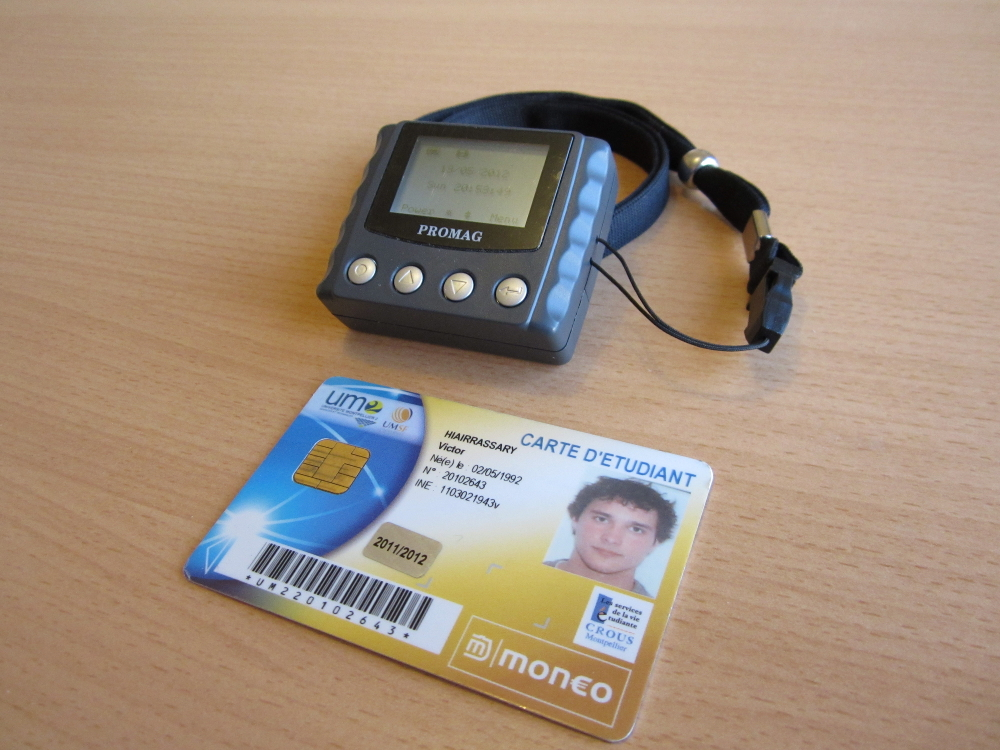
\includegraphics[scale=0.4]{images/mfr.jpg} 
        \end{center}
     \end{figure} 
\end{frame}


\begin{frame}{MFR120U - Inconvénients}
	\begin{block}{Inconvénients}
        Le module souffre de quelques inconvénients:

	    \begin{itemize}
            \item Logiciel d'exploitation disponible seulement sous Windows
            \item Nécessite un cable USB
            \item Pas assez intuitif à l'utilisation
            \item Besoin d'un driver sous Windows et MacOS X
	    \end{itemize}
	\end{block}
\end{frame}


\subsection{Caractère multi-plateforme}
\begin{frame}{Caractère multi-plateforme}
	\begin{block}{C++}
        Langage inévitable pour pouvoir dialoger de façon optimale sur une connection
        série/Bluetooh.

	    \begin{itemize}
            \item Multi-paradigmes
            \item Cross-platform, cross-compiler
            \item C++11
            \item Rapidité d'exécution
	    \end{itemize}
	\end{block}

	\begin{block}{CMake}
        Déploiement rapide d'un projet sur de multiples plateformes (Windows, Linux,
    MacOS X, etc) ainsi que plusieurs compilateurs (msvc, g++, clang++).
	\end{block}
\end{frame}


\subsection{Prototype}
\begin{frame}{Prototype}
	\begin{block}{Prototype}
        Rencontre avec M. Tamby début mars. Correction de beaucoup d'aspects négatifs,
        correspondant à nos besoins réels.
	\end{block}

    \begin{figure}[h]
        \begin{center}
            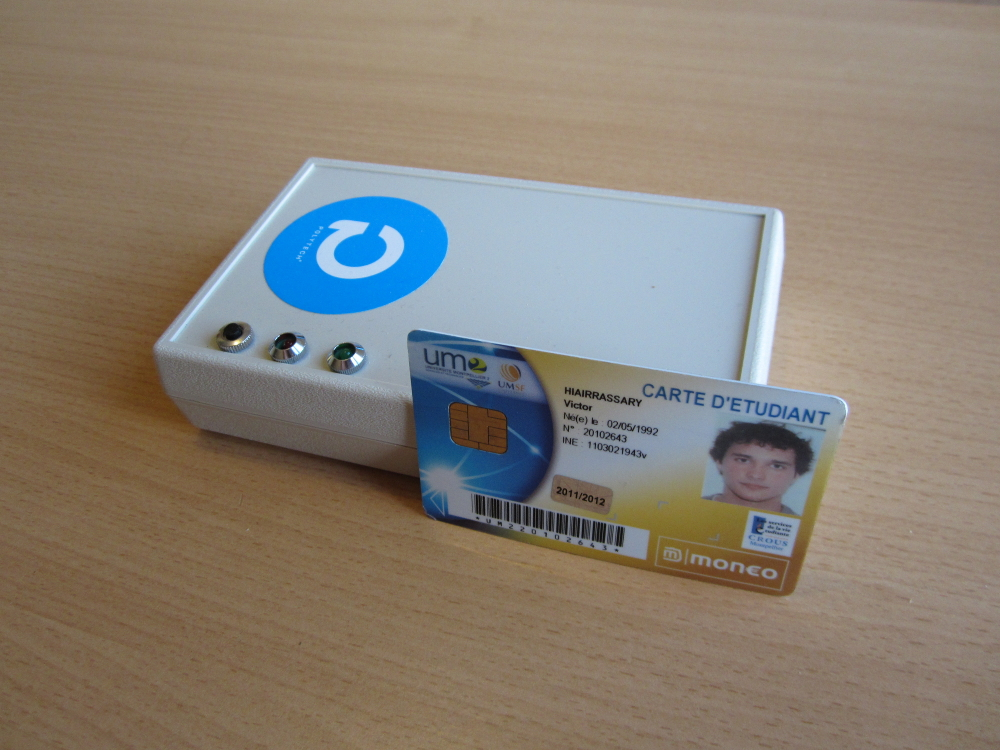
\includegraphics[scale=0.4]{images/proto.jpg} 
        \end{center}
     \end{figure} 
\end{frame}

\subsection{Prototype - Architecture matérielle}
\begin{frame}{Architecture matérielle}
	\begin{block}{Schéma}
        Schéma ``général'' du prototype. Aspect délibérement simplifié.
	\end{block}

    \begin{figure}[h]
        \begin{center}
            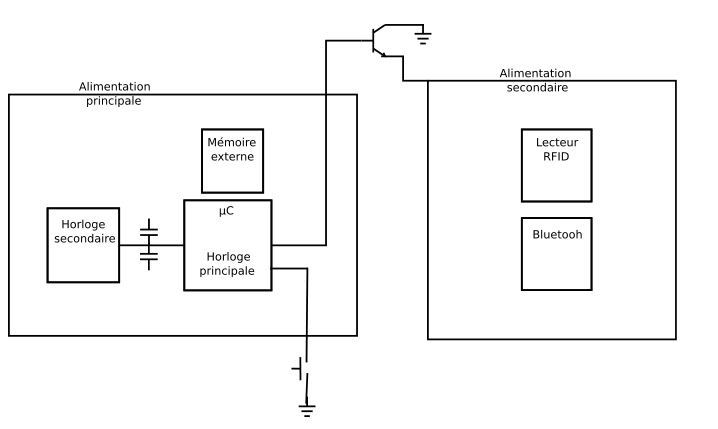
\includegraphics[scale=0.4]{images/protoSchema.png} 
        \end{center}
     \end{figure} 
\end{frame}
